\documentclass[tikz,border=12pt]{standalone}
\usepackage[T1]{fontenc}
\usepackage{mathpazo}
\usepackage{amsmath,amssymb}
\usetikzlibrary{arrows.meta, positioning, calc, fit, decorations.pathreplacing}

\definecolor{stblue}{HTML}{7B97AD}
\definecolor{rwgold}{HTML}{B8995E}
\definecolor{sage}{HTML}{7A9A7E}
\definecolor{dkbrown}{HTML}{3D3530}
\definecolor{wmgray}{HTML}{7B7067}
\definecolor{cream}{HTML}{F9F6F0}
\definecolor{border}{HTML}{D4C9B8}
\definecolor{terracotta}{HTML}{C47A6A}
\definecolor{lavender}{HTML}{907EA0}

\begin{document}
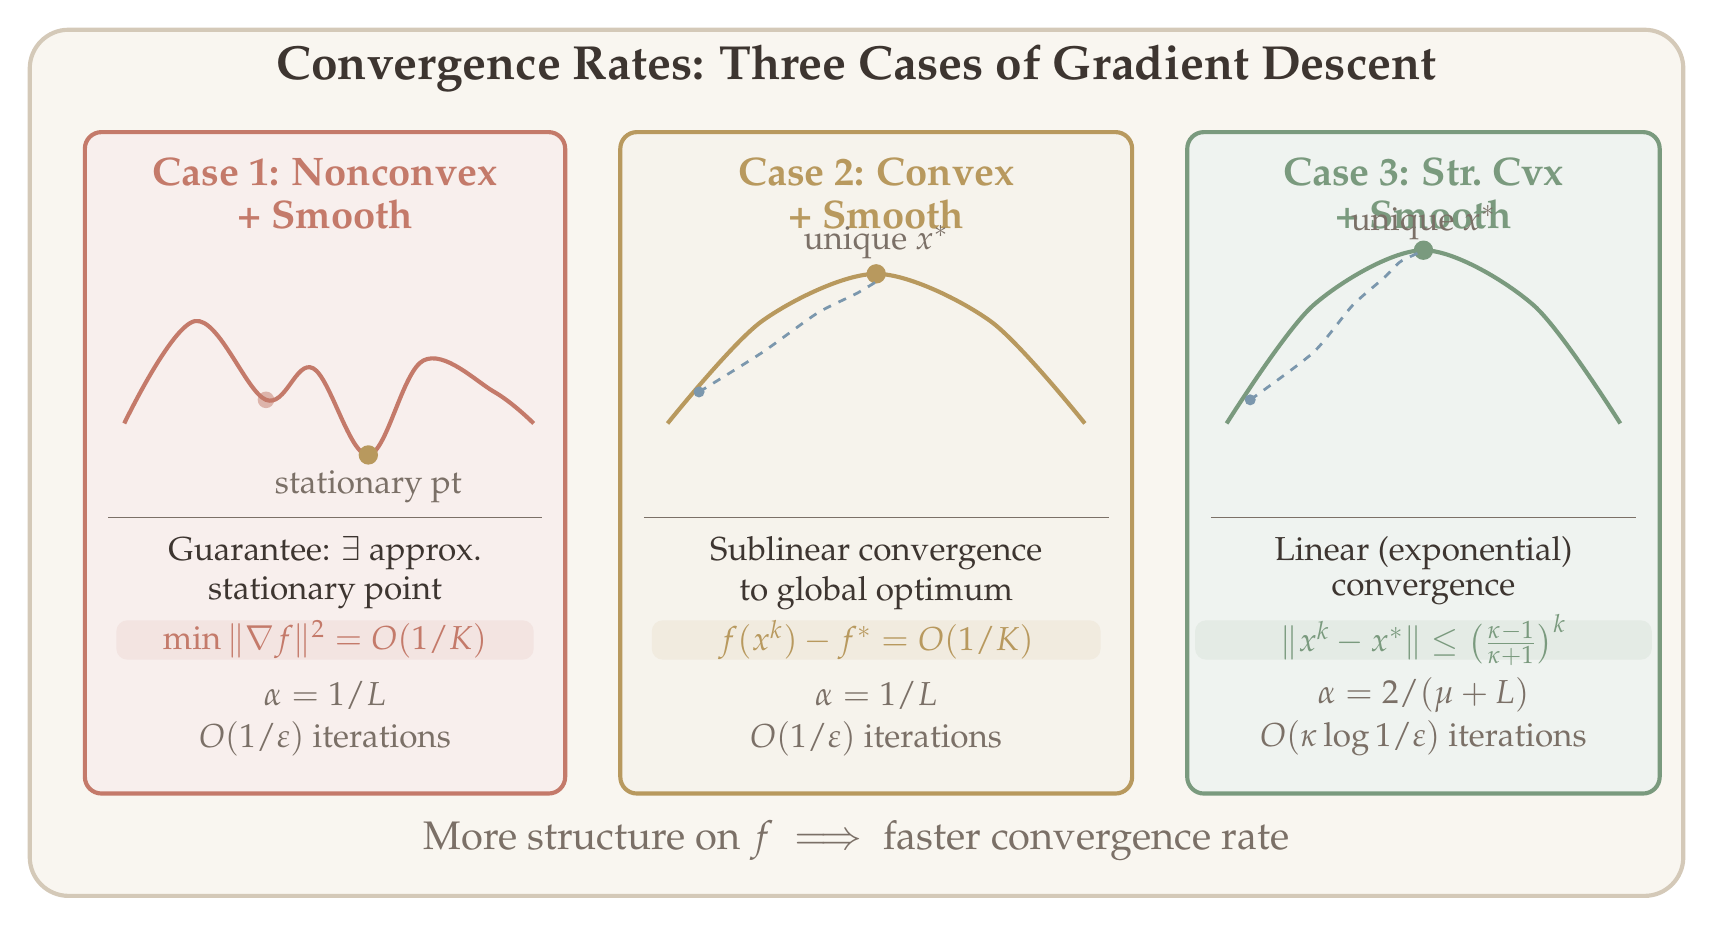
\begin{tikzpicture}[>={Stealth[length=4mm, width=3mm]}]

% Background
\fill[cream, rounded corners=14pt] (-0.5,-0.5) rectangle (20.5,10.5);
\draw[border, line width=1.5pt, rounded corners=14pt] (-0.5,-0.5) rectangle (20.5,10.5);

% Title
\node[text=dkbrown, font=\LARGE\bfseries] at (10,10.0) {Convergence Rates: Three Cases of Gradient Descent};

% --- Case 1: Nonconvex + Smooth ---
\fill[terracotta!12, rounded corners=6pt] (0.2,0.8) rectangle (6.3,9.2);
\draw[terracotta, line width=1.5pt, rounded corners=6pt] (0.2,0.8) rectangle (6.3,9.2);
\node[text=terracotta, font=\Large\bfseries] at (3.25,8.7) {Case 1: Nonconvex};
\node[text=terracotta, font=\Large\bfseries] at (3.25,8.15) {+ Smooth};

% Landscape with multiple local minima
\draw[terracotta, line width=1.5pt] plot[smooth, tension=0.6] coordinates {(0.7,5.5) (1.6,6.8) (2.5,5.8) (3.1,6.2) (3.8,5.1) (4.5,6.3) (5.4,5.9) (5.9,5.5)};
\fill[terracotta, opacity=0.5] (2.5,5.8) circle (3pt);
\fill[rwgold] (3.8,5.1) circle (3.5pt);
\node[text=wmgray, font=\large] at (3.8,4.7) {stationary pt};

\draw[wmgray, line width=0.4pt] (0.5,4.3) -- (6.0,4.3);

\node[text=dkbrown, font=\large] at (3.25,3.85) {Guarantee: $\exists$ approx.};
\node[text=dkbrown, font=\large] at (3.25,3.35) {stationary point};

\fill[terracotta!20, rounded corners=4pt] (0.6,2.5) rectangle (5.9,3.0);
\node[text=terracotta, font=\large] at (3.25,2.75) {$\min\|\nabla f\|^2 = O(1/K)$};

\node[text=wmgray, font=\large] at (3.25,2.05) {$\alpha = 1/L$};
\node[text=wmgray, font=\large] at (3.25,1.5) {$O(1/\varepsilon)$ iterations};

% --- Case 2: Convex + Smooth ---
\fill[rwgold!12, rounded corners=6pt] (7.0,0.8) rectangle (13.5,9.2);
\draw[rwgold, line width=1.5pt, rounded corners=6pt] (7.0,0.8) rectangle (13.5,9.2);
\node[text=rwgold, font=\Large\bfseries] at (10.25,8.7) {Case 2: Convex};
\node[text=rwgold, font=\Large\bfseries] at (10.25,8.15) {+ Smooth};

% Convex bowl
\draw[rwgold, line width=1.5pt] plot[smooth, tension=0.5] coordinates {(7.6,5.5) (8.8,6.8) (10.25,7.4) (11.7,6.8) (12.9,5.5)};
\fill[rwgold] (10.25,7.4) circle (3.5pt);
\node[text=wmgray, font=\large] at (10.25,7.8) {unique $x^*$};

% Staircase showing 1/K decay
\draw[stblue, line width=1pt, dashed] plot[smooth, tension=0.4] coordinates {(8.0,5.9) (8.8,6.4) (9.5,6.9) (10.0,7.15) (10.25,7.3)};
\fill[stblue] (8.0,5.9) circle (2pt);

\draw[wmgray, line width=0.4pt] (7.3,4.3) -- (13.2,4.3);

\node[text=dkbrown, font=\large] at (10.25,3.85) {Sublinear convergence};
\node[text=dkbrown, font=\large] at (10.25,3.35) {to global optimum};

\fill[rwgold!20, rounded corners=4pt] (7.4,2.5) rectangle (13.1,3.0);
\node[text=rwgold, font=\large] at (10.25,2.75) {$f(x^k) - f^* = O(1/K)$};

\node[text=wmgray, font=\large] at (10.25,2.05) {$\alpha = 1/L$};
\node[text=wmgray, font=\large] at (10.25,1.5) {$O(1/\varepsilon)$ iterations};

% --- Case 3: Strongly Convex + Smooth ---
\fill[sage!12, rounded corners=6pt] (14.2,0.8) rectangle (20.2,9.2);
\draw[sage, line width=1.5pt, rounded corners=6pt] (14.2,0.8) rectangle (20.2,9.2);
\node[text=sage, font=\Large\bfseries] at (17.2,8.7) {Case 3: Str.\ Cvx};
\node[text=sage, font=\Large\bfseries] at (17.2,8.15) {+ Smooth};

% Steep convex bowl
\draw[sage, line width=1.5pt] plot[smooth, tension=0.5] coordinates {(14.7,5.5) (15.8,7.0) (17.2,7.7) (18.6,7.0) (19.7,5.5)};
\fill[sage] (17.2,7.7) circle (3.5pt);
\node[text=wmgray, font=\large] at (17.2,8.05) {unique $x^*$};

% Exponential convergence staircase
\draw[stblue, line width=1pt, dashed] plot[smooth, tension=0.4] coordinates {(15.0,5.8) (15.8,6.4) (16.3,7.0) (16.7,7.35) (16.9,7.55) (17.1,7.65) (17.2,7.7)};
\fill[stblue] (15.0,5.8) circle (2pt);

\draw[wmgray, line width=0.4pt] (14.5,4.3) -- (19.9,4.3);

\node[text=dkbrown, font=\large] at (17.2,3.85) {Linear (exponential)};
\node[text=dkbrown, font=\large] at (17.2,3.35) {convergence};

\fill[sage!20, rounded corners=4pt] (14.3,2.5) rectangle (20.1,3.0);
\node[text=sage, font=\large] at (17.2,2.75) {$\|x^k - x^*\| \leq \bigl(\frac{\kappa-1}{\kappa+1}\bigr)^k$};

\node[text=wmgray, font=\large] at (17.2,2.05) {$\alpha = 2/(\mu + L)$};
\node[text=wmgray, font=\large] at (17.2,1.5) {$O(\kappa \log 1/\varepsilon)$ iterations};

% Bottom arrow
\node[text=wmgray, font=\Large] at (10,0.2) {More structure on $f$ $\;\Longrightarrow\;$ faster convergence rate};

\end{tikzpicture}
\end{document}
